\documentclass[notheorems]{beamer}

\usepackage{amsmath}
\usepackage{amssymb}
\usepackage[scale=2]{ccicons}
\usepackage{appendixnumberbeamer}
\usepackage{booktabs}
\usepackage[toc,page]{appendix}
\usepackage{graphicx}
\usepackage{xspace}
\usepackage{adjustbox, lipsum}
\usepackage{bbm}
\usepackage{algorithm}
\usepackage{algpseudocode}
\usepackage[sort,numbers]{natbib}

% absolute positioning
\usepackage[absolute,overlay]{textpos}

\newcommand{\source}[1]{{\let\thefootnote\relax\footnote{{\tiny #1}}}}

\input{macros/math}
\usepackage{simplebeam}

\title{Better Optimization via Interpolation}
\author{Aaron Mishkin}
\institute{}
\date{}


\begin{document}

    \setbeamercolor{background canvas}{bg=lightcyan}
        \begin{frame}
        \vspace{1em}
    % \begin{frame}{Research Outlook}
        \begin{center}
            {\Large \textbf{Painless Stochastic Gradient Descent}: Interpolation, Line-Search, and Convergence Rates. \vspace{1em}}


            {\large NeurIPS 2019 \vspace{0.5em} }

            {\large Aaron Mishkin }
        \end{center}

        \vspace{2.5em}

        \begin{figure}
            \centering
            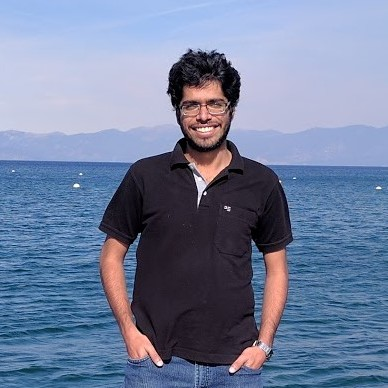
\includegraphics[width=0.18\textwidth]{collaborators/sharan}
            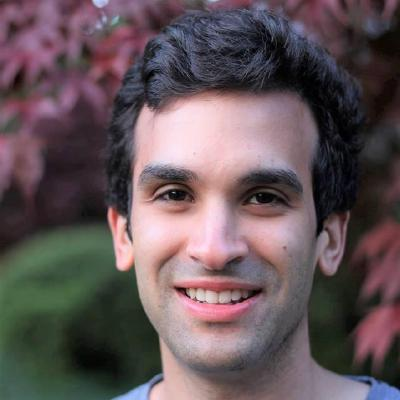
\includegraphics[width=0.18\textwidth]{collaborators/issam}
            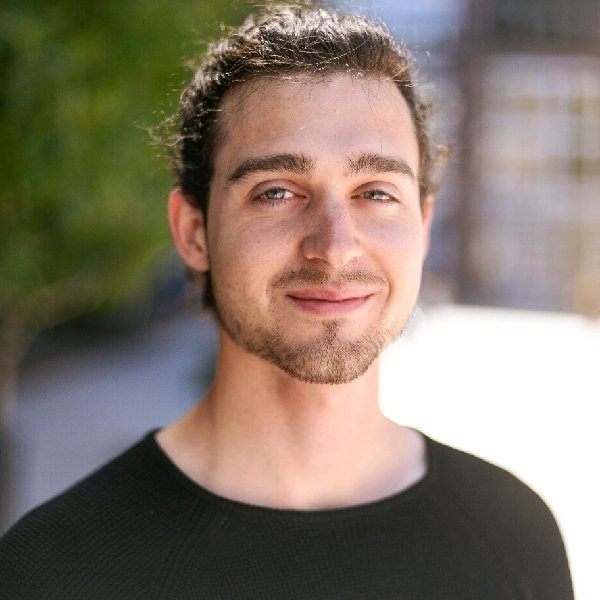
\includegraphics[width=0.18\textwidth]{collaborators/gauthier}
            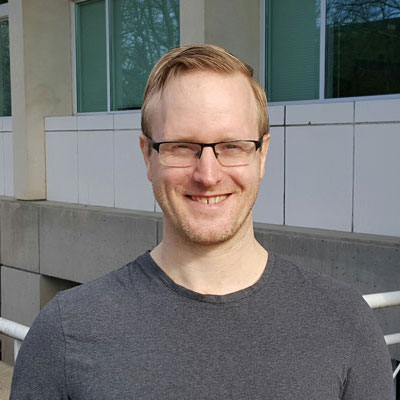
\includegraphics[width=0.18\textwidth]{collaborators/mark}
            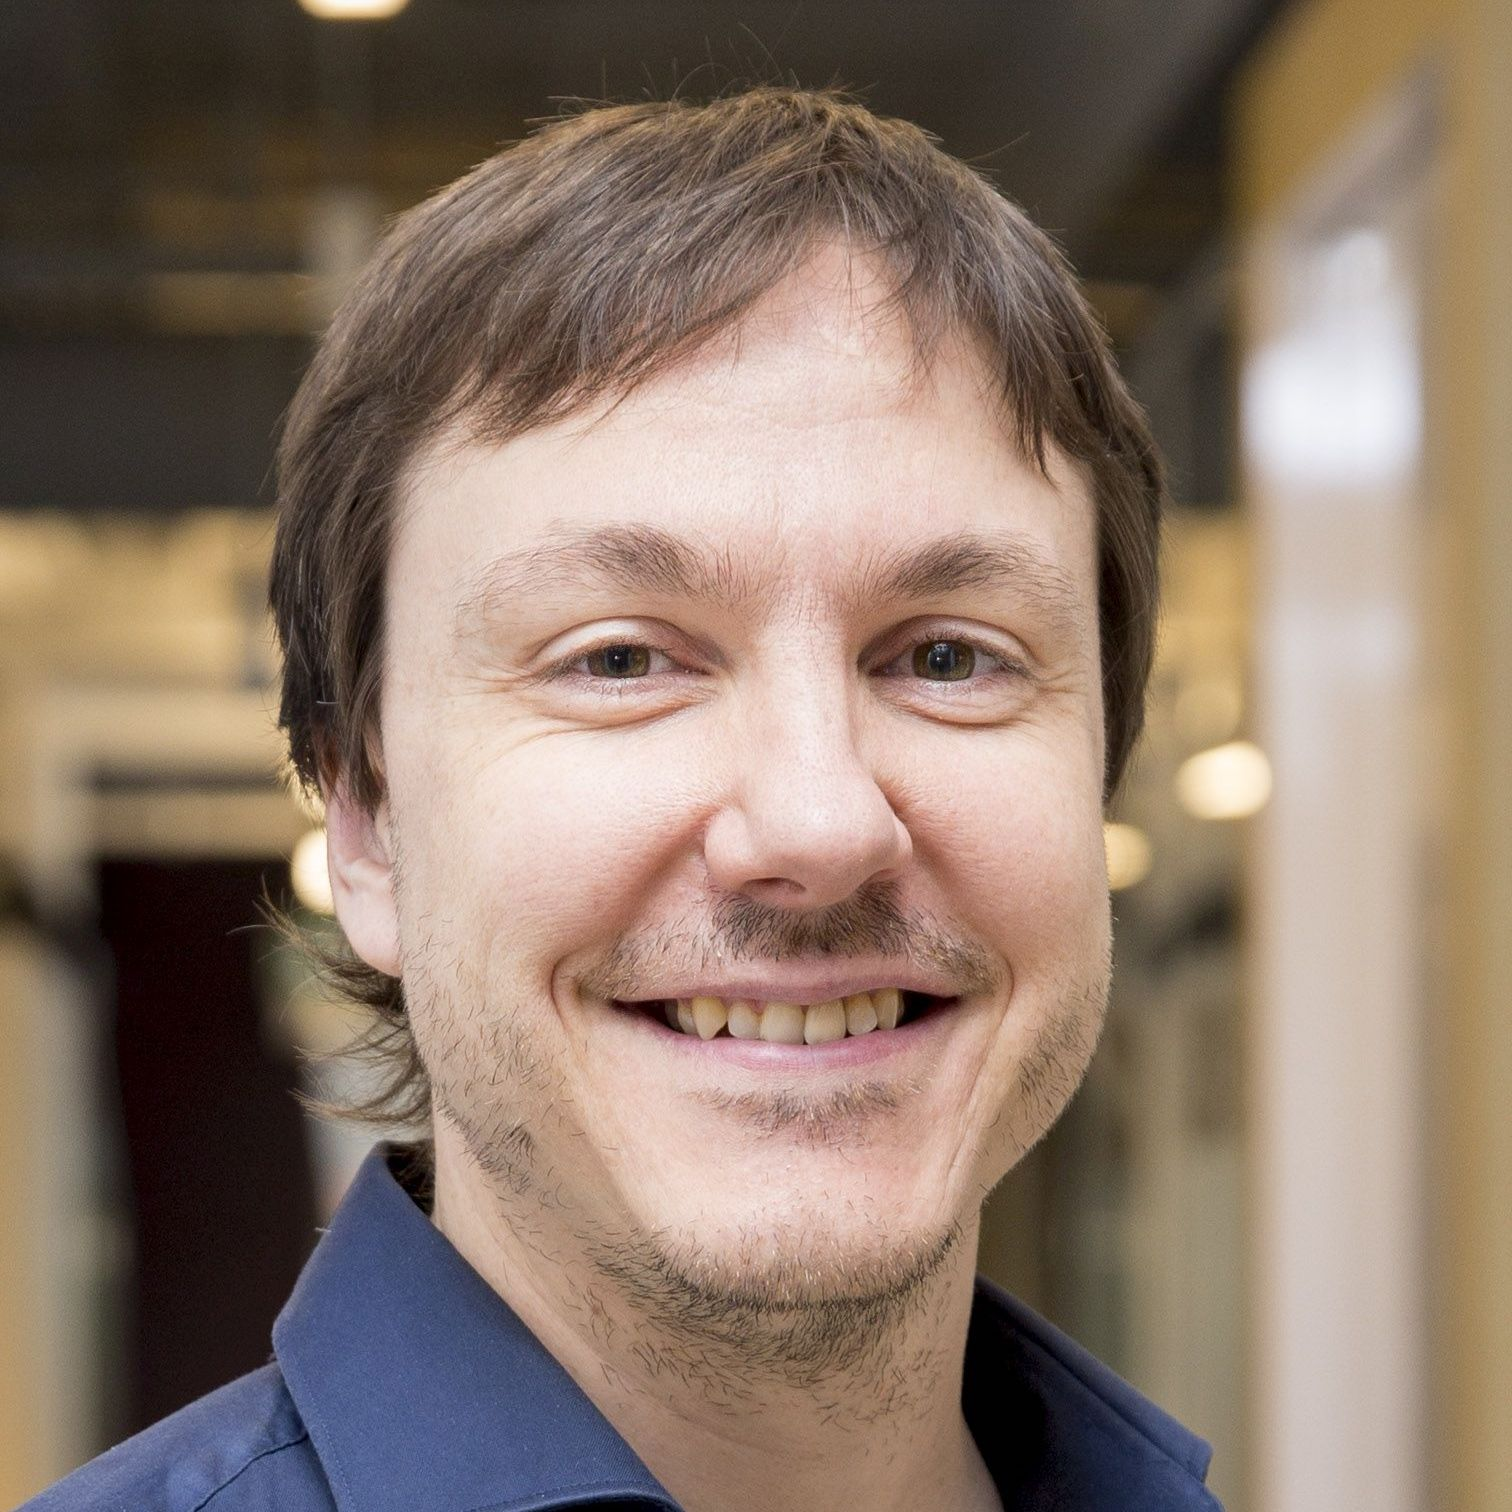
\includegraphics[width=0.18\textwidth]{collaborators/simon}
        \end{figure}

        % \vspace{1cm}
        %
        % { \Large
        % This requires
        % \begin{minipage}[t]{\textwidth}
        %     % \vspace{-0.27cm}%
        %     \centering
        %     \begin{enumerate}
        %         \item developing parameter-free algorithms;
        %         \item proving correctness and convergence rates;
        %         \item making statistical trade-offs explicit.
        %     \end{enumerate}
        % \end{minipage}
        %
        % }

    \end{frame}
    \setbeamercolor{background canvas}{bg=white}

    \begin{frame}{Stochastic Gradient Descent: Workhorse of ML?}

        \begin{center}
            \Large
            ``Stochastic gradient descent (SGD) is today one of the main workhorses for solving large-scale supervised learning and optimization problems.''\\
            ---\citet{drori2019complexity}
        \end{center}

    \end{frame}

    \begin{frame}{Consensus Says\ldots}

        \begin{center}
            \Large \dots and also ~\citet{xu2017second,
            zhang2016parallel,
            patterson2017deep,
            pillaud2018statistical,
            grosse2015scaling,
            assran2018stochastic,
            damaskinos2019aggregathor,
            kawaguchi2020ordered,
            bernstein2018signsgd,
            li2019rsa,
            agarwal2017second,
            hofmann2015variance,
            geffner2019rule,
            assran2020convergence,
            gower2019sgd}
        \end{center}

    \end{frame}

    \begin{frame}{Motivation: Challenges in Optimization for ML}

        \textbf{Stochastic gradient methods} are the most popular algorithms for fitting ML models,
        \begin{align*}
            \textbf{SGD:} \quad w_{k + 1} = w_k - \eta_k \nabla \tilde{f} \, (w_k). \\
        \end{align*}

        % SGD is scalable and converges if $\eta_k$ decreases sufficiently slowly.\vspace{1em}

        But practitioners face major challenges with \vspace{0.5em}
        \begin{itemize}
            \item \textbf{Speed}: step-size/averaging controls convergence rate.
            \item \textbf{Stability}: hyper-parameters must be tuned carefully.
            \item \textbf{Generalization}: optimizers encode statistical tradeoffs.
        \end{itemize}
        \vspace{1em}

    \end{frame}

    \begin{frame}{Better Optimization via Better Models}

        \begin{figure}
            \centering
            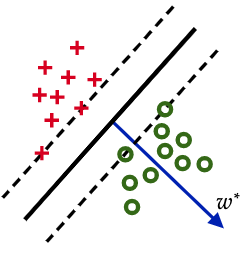
\includegraphics[width=0.38\textwidth]{figures/separable}
            \hspace{0.2em}
            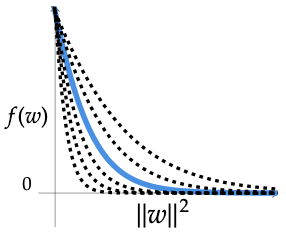
\includegraphics[width=0.45\textwidth]{figures/loss_fn}
        \end{figure}
        \vspace{0.2em}

        \begin{center}
            \large \textbf{Idea}: exploit model properties for better optimization.\vspace{0.25em}
        \end{center}

            % \begin{minipage}[]{.55\textwidth}
            %     \textbf{Path Forward}: exploit properties of models to design better optimizers.\vspace{1em}
            %
            %     Consider minimizing
            %     \[ f \,(w) = \sum_{i=1}^n f_i(w). \]
            %     We say $f$ satisfies \textbf{interpolation} if $\forall w$,
            %     \begin{align*}
            %         f\,(w^*) \leq f\,(w) \implies f_i(w^*) \leq f_i(w).
            %     \end{align*}
            %  \end{minipage} %
            %  \hfill%clean
            % \begin{minipage}[]{.4\textwidth}
            %     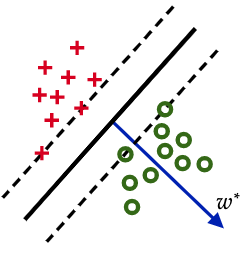
\includegraphics[width=\textwidth]{figures/separable}\vspace{-0.5cm}
            %     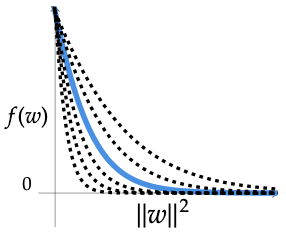
\includegraphics[width=1.1\textwidth]{figures/loss_fn}
            % \end{minipage}

    \end{frame}

    \begin{frame}{Interpolation}
        \[ \textbf{Loss:} \quad f \,(w) = \frac{1}{n}\sum_{i=1}^n f_i(w). \]

        \textbf{Interpolation} is satisfied for \( f \) if $\forall w$,
        \begin{align*}
            f\,(w^*) \leq f\,(w) \implies f_i(w^*) \leq f_i(w).\\
        \end{align*}

        {\hspace{0.125\textwidth} \large{\textbf{Separable} \hspace{0.3\textwidth} \textbf{Not Separable}}}
        \begin{figure}
            \centering
            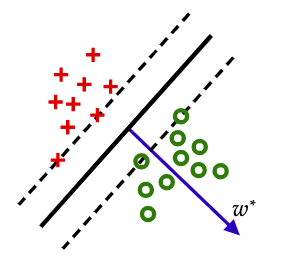
\includegraphics[width=0.4\textwidth]{figures/separable_2}
            \hspace{0.1\textwidth}
            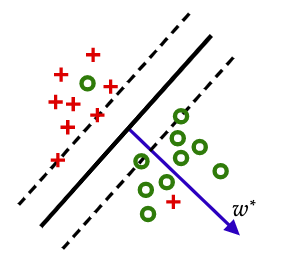
\includegraphics[width=0.4\textwidth]{figures/not_separable_2}
        \end{figure}

    \end{frame}

    \begin{frame}{Constant Step-size SGD}

        Interpolation and smoothness imply a \textbf{noise bound},
        \begin{align*}
            \E \norm{\nabla f_i (w)}^2 \leq \rho \rbr{f\,(w) - f\,(w^*)}.
        \end{align*}

        \begin{itemize}
            \item SGD converges with a \textbf{constant step-size}~\citep{vaswani2019fast, bassily2018exponential}.
            \item SGD is (nearly) as \textbf{fast} as gradient descent.
            \item SGD converges to the
            \begin{itemize} \normalsize
                \item minimum L$_2$-norm solution for linear regression~\citep{wilson2017marginal}.
                \item max-margin solution for logistic regression~\citep{nacson2018stochastic}.
                \item ??? for deep neural networks.\vspace{1em}
            \end{itemize}
        \end{itemize}

        \textbf{Takeaway}: optimization speed and (some) statistical trade-offs.\\
        \vspace{0.1cm}

    \end{frame}

    \begin{frame}{Painless SGD}

        \begin{center}
            {\huge What about \textbf{stability} and \textbf{hyper-parameter} tuning?}

            \vspace{2em}
            {\Large Is grid-search the best we can do?}
            \vspace{2em}
        \end{center}

        \begin{figure}
            \makebox[\textwidth][c]{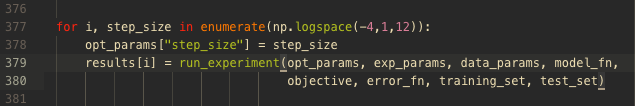
\includegraphics[width=1.1\textwidth]{figures/grid_search}}%
        \end{figure}

    \end{frame}

    \begin{frame}{Painless SGD: Tuning-free SGD via Line-Searches}

        \[ \textbf{Stochastic Armijo Condition}: \; f_i(w_{k+1}) \leq f_i(w_k) - c \, \eta_k \norm{\nabla f_i(w_k)}^2. \]
        \begin{figure}
            \centering
            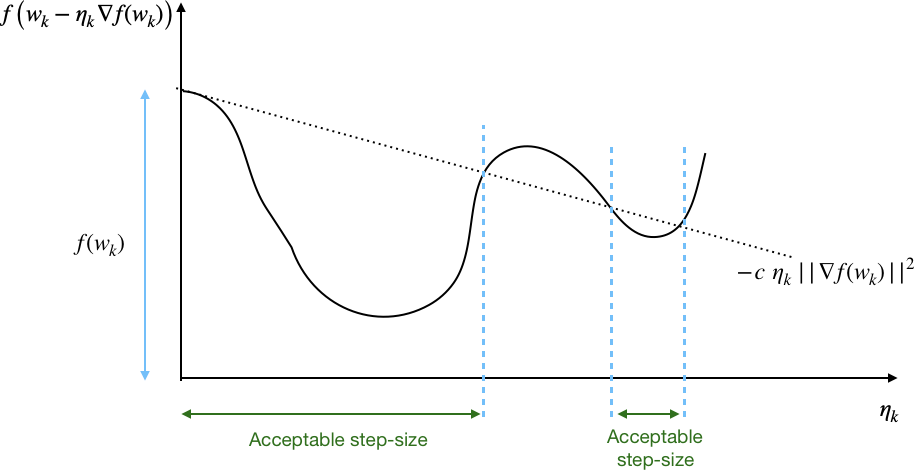
\includegraphics[width=\textwidth]{figures/armijo}
        \end{figure}

    \end{frame}

    \begin{frame}{Painless SGD: Stochastic Armijo in Theory}
        \begin{figure}
            \makebox[\textwidth][c]{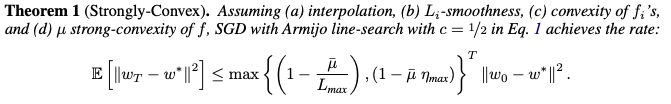
\includegraphics[width=1\textwidth]{theory/sc}}
            \vspace{0.5em}

            \makebox[\textwidth][c]{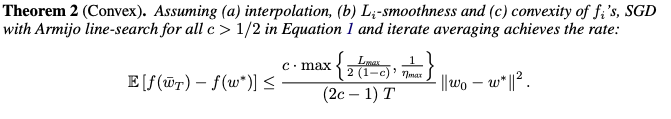
\includegraphics[width=1\textwidth]{theory/c}}
            \vspace{0.5em}

            \makebox[\textwidth][c]{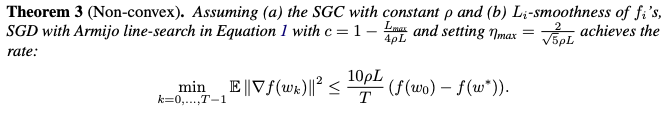
\includegraphics[width=1\textwidth]{theory/nc}}
        \end{figure}
    \end{frame}

    \begin{frame}{Painless SGD: Stochastic Armijo in Practice}

        {\large Classification accuracy for ResNet-34 models trained on MNIST, CIFAR-10, and CIFAR-100. }\vspace{0.5em}

        \begin{figure}
            \centering
            \makebox[\textwidth][c]{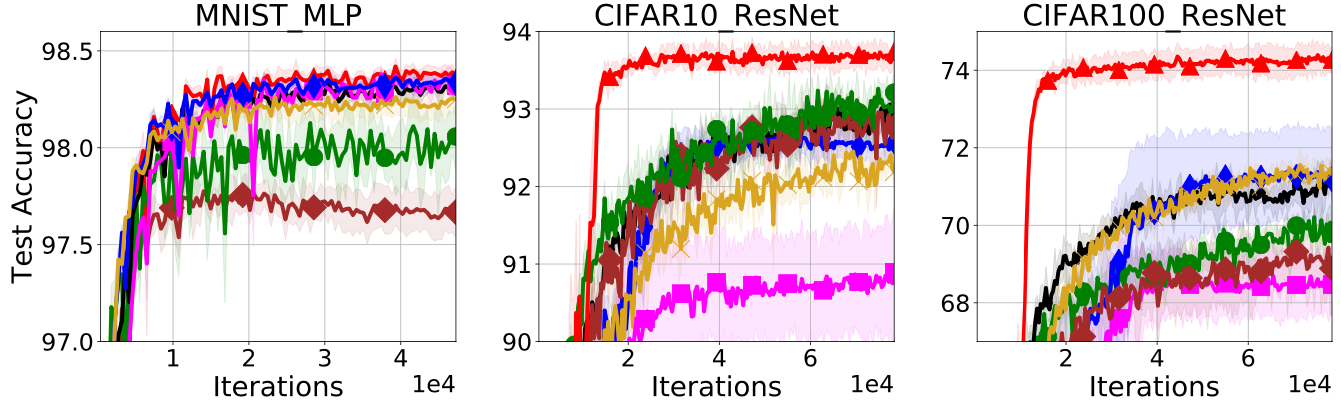
\includegraphics[width=1.1\textwidth]{figures/sls}}\vspace{0.5em}
            \makebox[\textwidth][c]{
\includegraphics[width=1.1\textwidth]{figures/legend}}%
        \end{figure}

    \end{frame}

    \begin{frame}{Painless SGD: Added Cost}
        \textbf{Backtracking} is low-cost and averages once per-iteration.
        \begin{figure}
            \makebox[\textwidth][c]{
            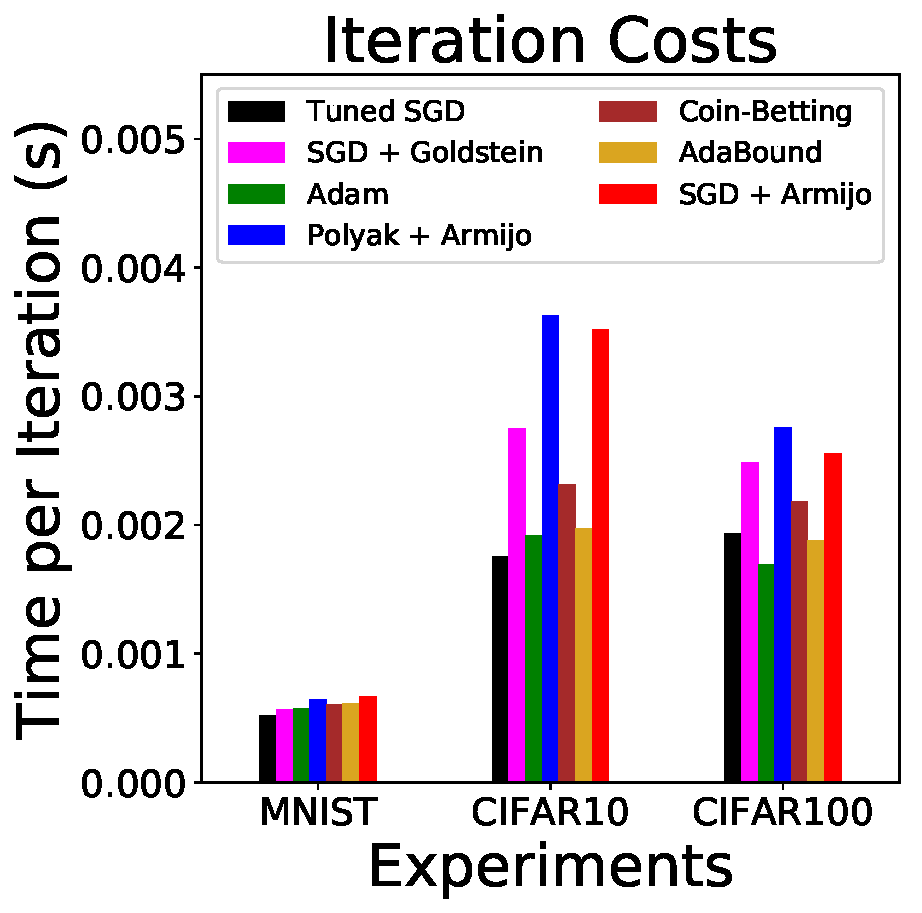
\includegraphics[width=0.55\textwidth]{figures/T}
            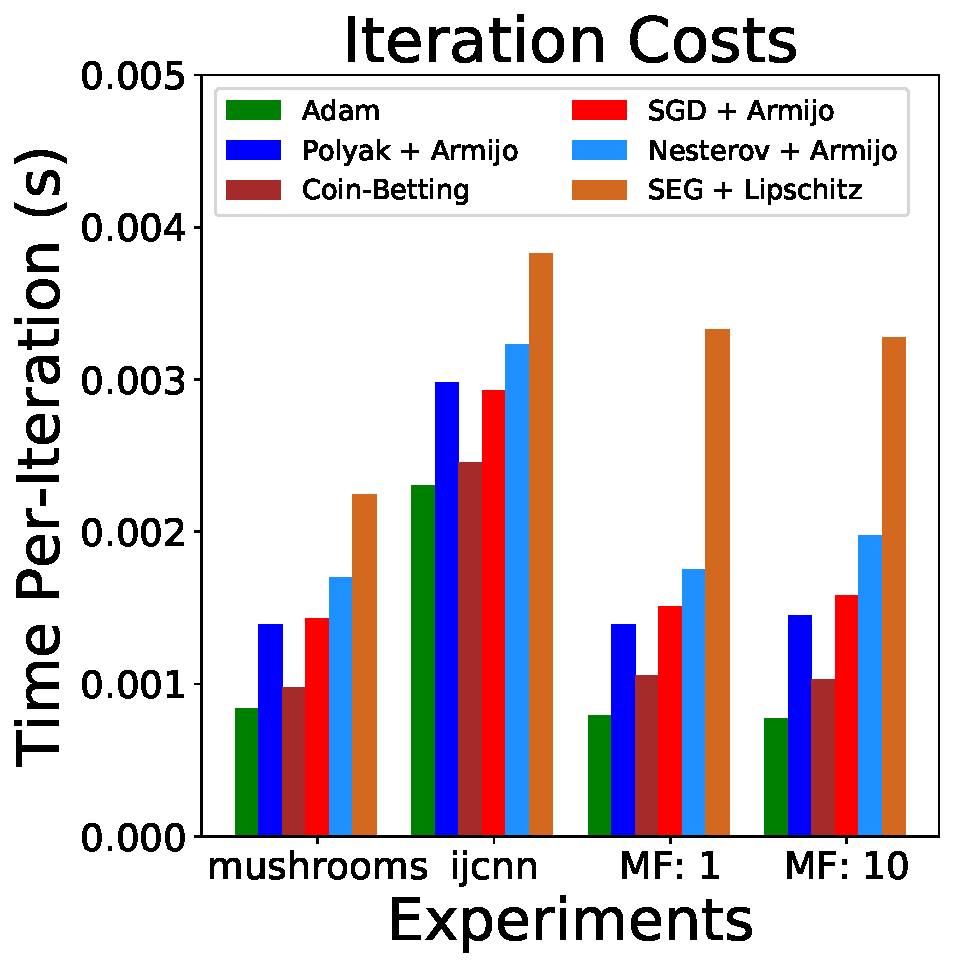
\includegraphics[width=0.55\textwidth]{figures/kernel_mf_runtimes}
            }
        \end{figure}

    \end{frame}


    \begin{frame}{Painless SGD: Sensitivity to Assumptions}

        SGD with line-search is \textbf{robust}, but can still fail catastrophically.

        \begin{figure}
            \makebox[\textwidth][c]{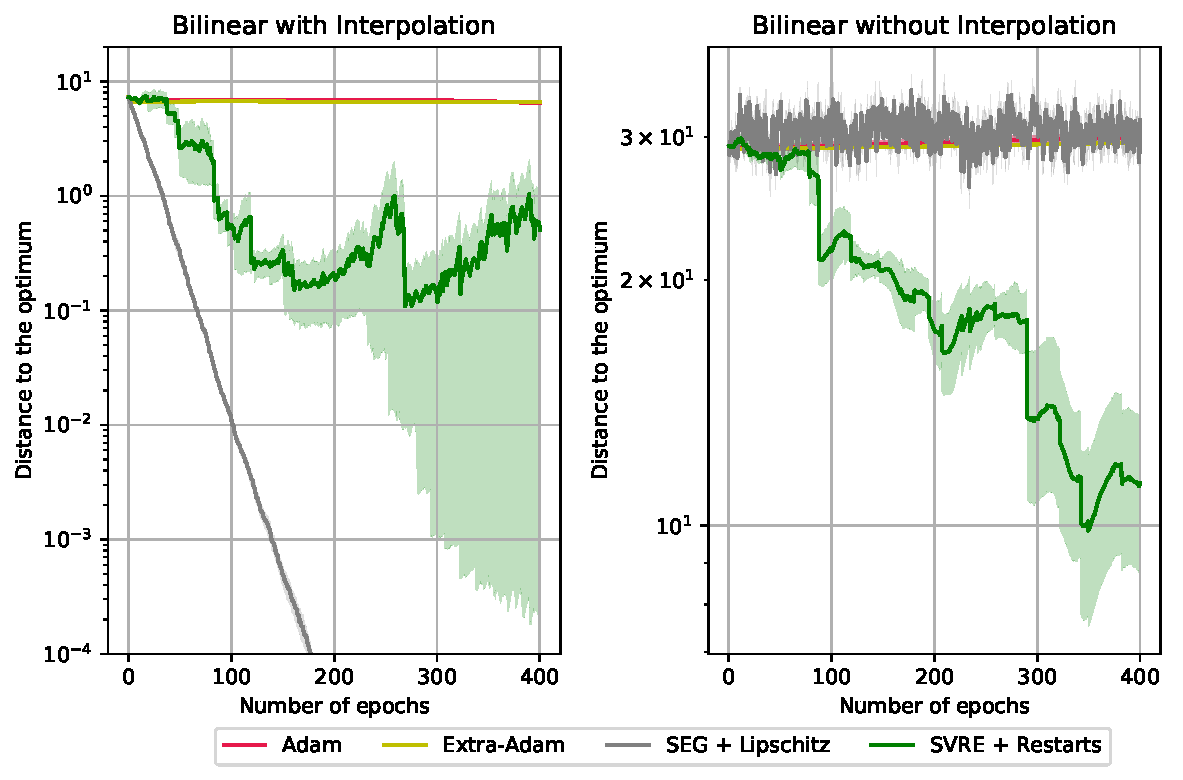
\includegraphics[width=0.98\textwidth]{figures/M}}
        \end{figure}

    \end{frame}

    \setbeamercolor{background canvas}{bg=lightcyan}

    \begin{frame}{}
        \begin{center}
        \huge Questions.
        \end{center}
    \end{frame}
    \setbeamercolor{background canvas}{bg=white}

    \begin{frame}{Bonus: Robust Acceleration for SGD}

        \begin{figure}[b]
            \centering
            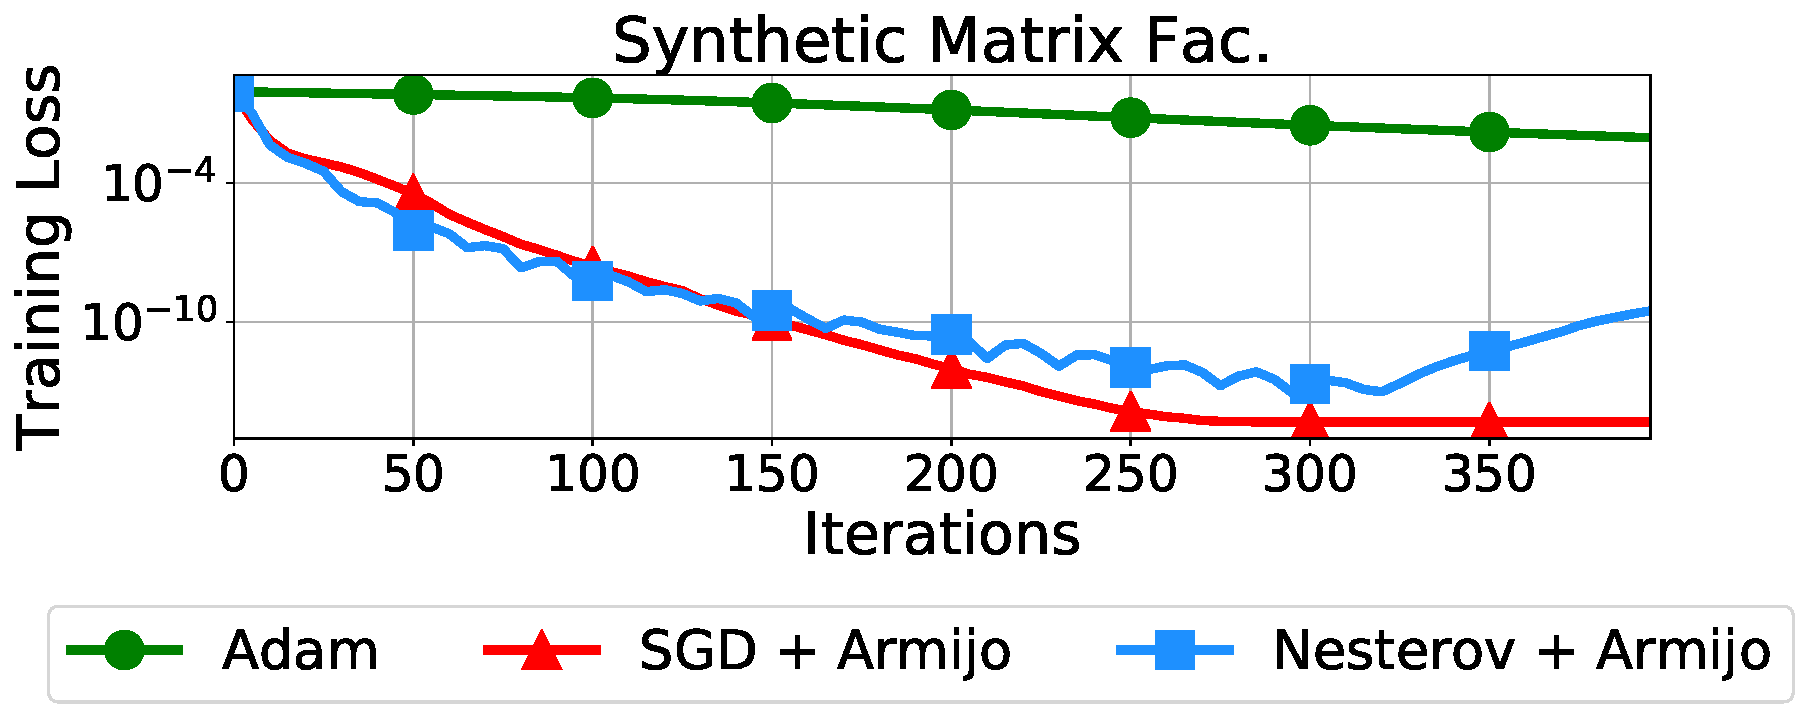
\includegraphics[width=0.9\textwidth]{figures/matrix_fac}
        \end{figure}

        \textbf{Stochastic acceleration} is possible~\citep{vaswani2019fast, liu2020accelerating}, but
        \begin{itemize}
            \item it's \textbf{unstable} with the backtracking Armijo line-search; and
            \item the "momentum" parameter must be \textbf{fine-tuned}.\vspace{0.2em}
        \end{itemize}

        \textbf{Potential Solutions:}
        \begin{itemize}
            \item more sophisticated line-search (e.g. FISTA~\citep{DBLP:journals/siamis/BeckT09}).
            \item stochastic restarts for oscillations.
        \end{itemize}

    \end{frame}

    % bibliography

    \begin{frame}[allowframebreaks]{References}
        \bibliographystyle{plainnat}
        \bibliography{refs}
    \end{frame}

\end{document}
